%!Tex Root = ../main.tex
% ./Packete.tex
% ./Design.tex
% ./Deklarationen.tex
% ./Vorbereitung.tex
% ./Aufgabe1.tex
% ./Aufgabe3.tex
% ./Aufgabe4.tex
% ./Appendix.tex

\section{Exercise 2}

\setcounter{exercise}{1}

\begin{frame}[t]{Aufgabe \thesection}{\small Maximum Matching, Minimum Vertex Cover, Maximum Indepedant Set, Minimum Edge Cover\vspace{0.5cm}}
  \begin{columns}
    \begin{column}[t]{0.25\textwidth}
      \resizebox{\textwidth}{!}{
        \begin{minipage}[t]{5cm}
          \ctikzfig{bipartite} 
        \end{minipage}
      }
      \begin{itemize}
        \item $\alpha'(B) = 5$\only<2>{\footnote[1]{\tiny finding an augmenting path and making the endpoints saturated}}
      \end{itemize}
    \end{column}
    \begin{column}[t]{0.25\textwidth}
      \resizebox{\textwidth}{!}{
        \begin{minipage}[t]{5cm}
          \ctikzfig{bipartite_2}
        \end{minipage}
      }
      \begin{itemize}
        \item $\beta(B) = 5$\only<2>{\footnote[2]{\tiny dual property of the maximum matching: if one starts a search from the unmatched vertices on side A and one doesn't find an augmenting path, one can find a minimum vertex cover by taking the vertices on side B one does see, together with the vertices on side A one doesn't see}}
          % There can't be an uncovered edge - which would go from a vertex on side A you do see from a vertex on side B you don't see - because then that vertex on side B would become one of the ones you do explore
      \end{itemize}
    \end{column}
    \begin{column}[t]{0.25\textwidth}
      \resizebox{\textwidth}{!}{
        \begin{minipage}[t]{5cm}
          \ctikzfig{bipartite_3}
        \end{minipage}
      }
      \begin{itemize}
        \item $\alpha(B) = 7$\only<2>{\footnote[3]{\tiny the complement of a maximum independent set is a minimum vertex cover.}}
      \end{itemize}
    \end{column}
    \begin{column}[t]{0.25\textwidth}
      \resizebox{\textwidth}{!}{
        \begin{minipage}[t]{5cm}
          \ctikzfig{bipartite_4}
        \end{minipage}
      }
      \begin{itemize}
        \item $\beta'(B) = 7$\only<2>{\footnote[3]{\tiny finding a maximum matching and extending it greedily so that all vertices are covered}}
      \end{itemize}
    \end{column}
  \end{columns}
\end{frame}

\begin{frame}{Aufgabe \thesection}{Finding a minimum vertex cover}
  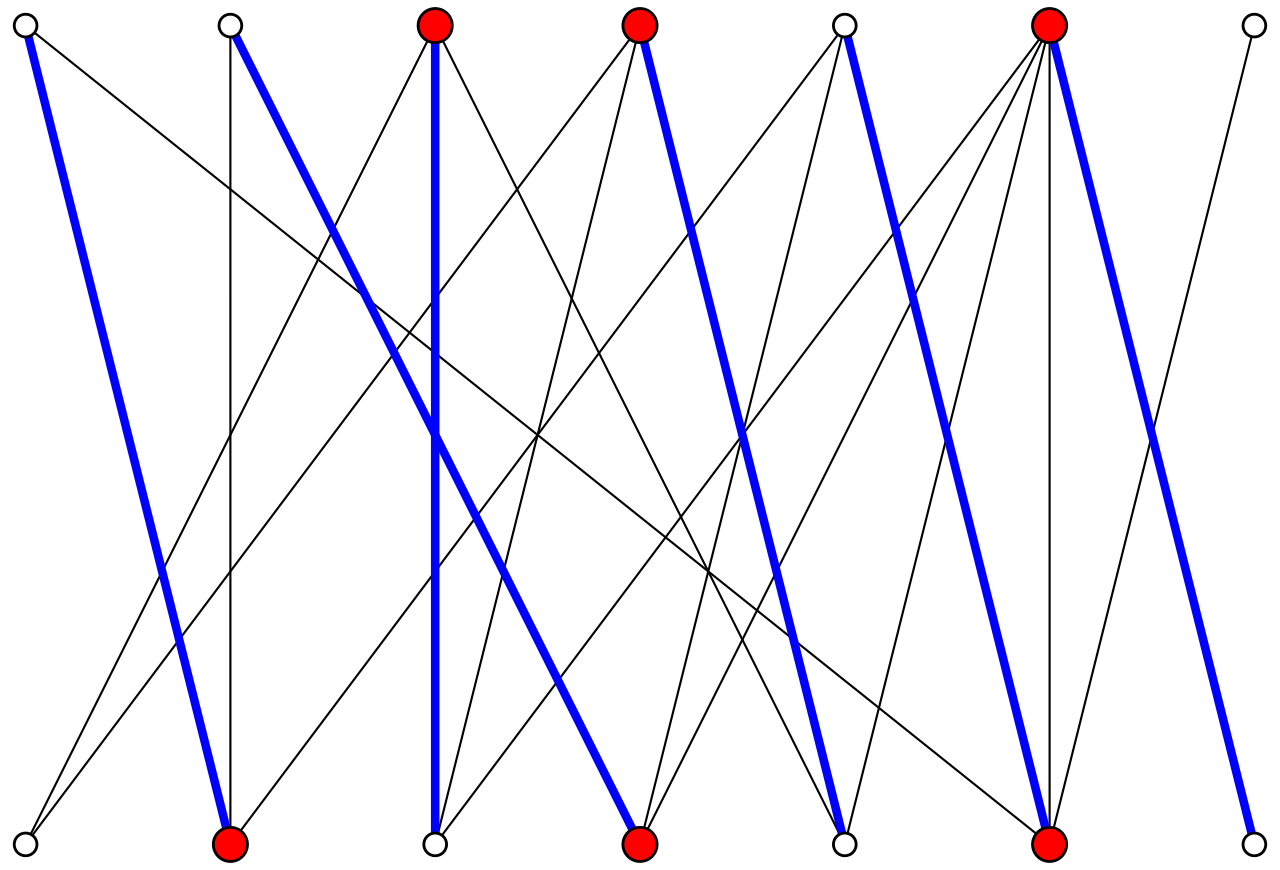
\includegraphics[height=0.5\paperheight, center]{./figures/vertex_cover_example.png}
\end{frame}

% https://math.stackexchange.com/questions/3074734/identifying-a-maximum-matching-and-a-minimum-cover-for-a-specific-bipartite-grap
% (In general, in a graph with bipartition (A,B) if you start a search from the unmatched vertices on side A, and you don't find an augmenting path, you can find a minimum vertex cover by taking the vertices on side B you do see, together with the vertices on side A you don't see. There can't be an uncovered edge - which would go from a vertex on side A you do see from a vertex on side B you don't see - because then that vertex on side B would become one of the ones you do explore.)
